\documentclass[table]{beamer}
\usepackage{ctex}
\usepackage{scrextend}
\usepackage{hyperref}
\usepackage[backend=bibtex, style=authoryear]{biblatex}
\usepackage{xcolor}
\usepackage{minted}

\addbibresource{ref.bib}
\usetheme{Madrid}

\title{深度学习的图像应用}
\subtitle{Deep Learning for Image Application}
\author{Garry}
\institute{大数据部门}
\date{\today}

\begin{document}
%%-------------------------------------------------
\frame{\titlepage}
%%-------------------------------------------------
\begin{frame}{概要}
	\tableofcontents
\end{frame}
%%-------------------------------------------------
\section{从零实现一个神经网络}
\begin{frame}
	\begin{center}
		\vspace{0.1cm}
		\Huge{从零实现一个神经网络}
	\end{center}
\end{frame}
\subsection{生成数据集}
\begin{frame}[fragile]
	\frametitle{数据集}
	\begin{figure}
		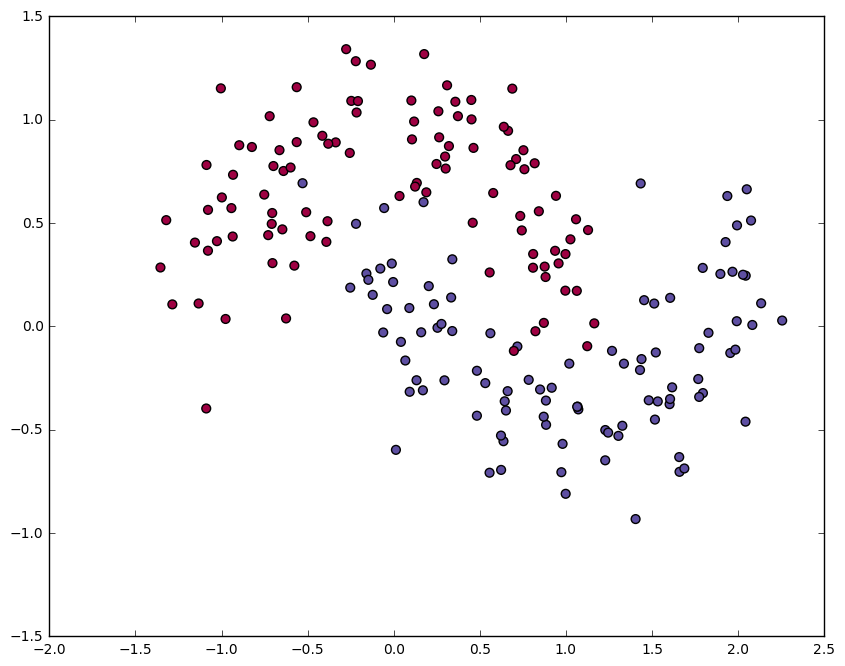
\includegraphics[width=0.5\textwidth]{generate_dataset.png}
		\caption{生成数据集}
		\label{fig:dataset}
	\end{figure}
  \begin{center}
    \begin{minipage}{0.8\textwidth}
		% 解决 beamer 中使用 minted出现的问题: http://nochair.net/posts/2011/05-05-fragile-latex-beamer.html
		% frame 环境加上 fragile 选项, 且\end{frame}必须独立放在一行.
		\definecolor{bg}{rgb}{0.95,0.95,0.95}
    \begin{minted}[bgcolor=bg,fontsize=\tiny]{python}
    # Generate a dataset and plot it
    np.random.seed(0)
    X, y = sklearn.datasets.make_moons(200, noise=0.20)
    plt.scatter(X[:,0], X[:,1], s=40, c=y, cmap=plt.cm.Spectral)
    \end{minted}
    \end{minipage}
  \end{center}
\end{frame}
\subsection{训练神经网络}
\begin{frame}
	\frametitle{网络结构}
	\begin{figure}
		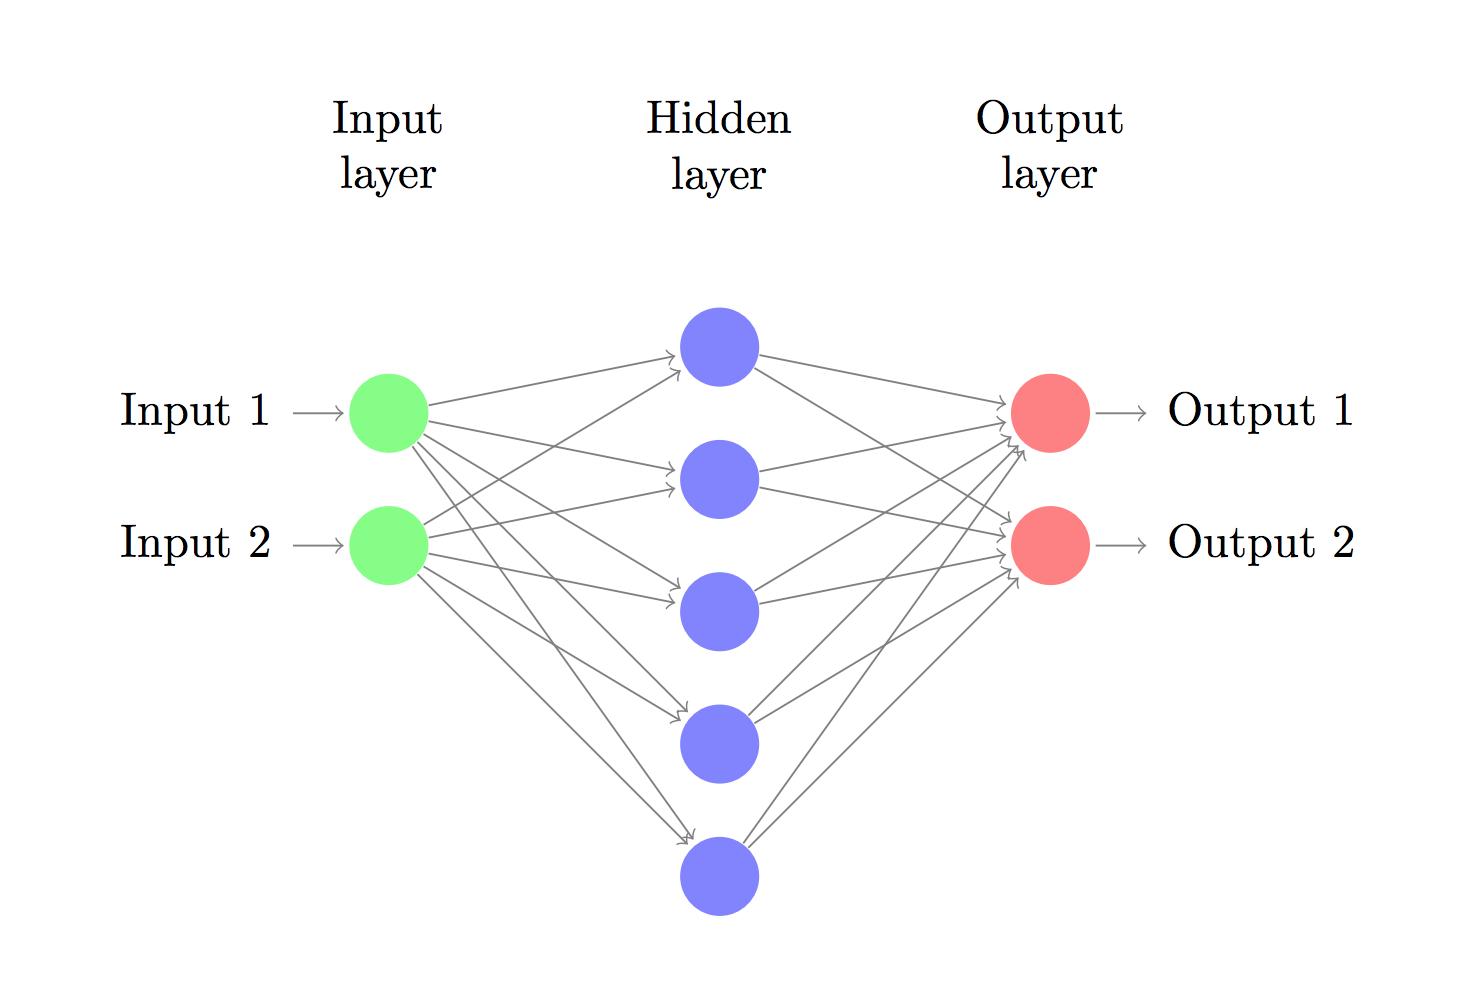
\includegraphics[width=0.5\textwidth]{nn-from-scratch-3-layer-network.png}
		\caption{网络结构}
		\label{fig:nn}
	\end{figure}
	建立一个三层的神经网络(一个输入层,一个隐藏层,一个输出层).输入层的维度由我们的数据决定.同样的, 输出层的维度由类别的个数决定.
\end{frame}

\subsection{预测}
\begin{frame}
	\frametitle{我们的网络如何预测?}
	\begin{equation}
		\begin{split}
			z_1 &= xW_1 + b_1\\
			a_1 &= \tanh(z_1)\\
			z_2 &= a_1W_2 + b_2\\
			a_2 &= \hat{y}=\mathrm{softmax}(z_2)
		\end{split}
	\end{equation}
	% 权重加在边上
	\begin{itemize}
		\item $z_i$ 表示第 $i$ 层的输入\footnote{$i$从0开始计数}
		\item $a_i$ 表示第 $i$ 层经过激活函数运算后的输出
		\item $W_1$,$b_1$,$W_2$,$b_2$ 是我们网络的参数,也就是我们要从训练网络中学习的
	\end{itemize}
	如果我们的隐藏层有500个节点, 则$W_1 \in \mathbb{R}^{2 \times 500}$, $b_1 \in \mathbb{R}^{500}$, $W_2 \in \mathbb{R}^{500 \times 2}$, $b_2 \in \mathbb{R}^2$.
\end{frame}
\begin{frame}
	\frametitle{学习参数}
	如果有$N$个训练样本, $C$个类别, 则我们预测的$\hat{y}$关于实际类别$y$的损失如下:
	\begin{equation}
		L(y,\hat{y})=-\frac{1}{N}\sum_{n \in N}\sum_{i \in C}{y_{n,i}\log{\hat{y}_{n,i}}}
	\end{equation}
	我们的目标是找到是损失函数最小的参数.
\end{frame}
\begin{frame}
	\frametitle{梯度下降}
	使用梯度下降(gradient descent)来寻找最小值.\\
	损失函数关于参数的梯度(导数): $\frac{\partial L}{\partial W_2}, \frac{\partial L}{\partial b_2}, \frac{\partial L}{\partial W_1}, \frac{\partial L}{\partial b_1}$.
	\begin{equation}
		\begin{split}
			\delta_3 &= \hat{y} - y\\
			\delta_2 &= (1-\tanh^2z_1)*\delta_3W^T_2\\
			\frac{\partial L}{\partial W_2} &= a^T_1\delta_3\\
			\frac{\partial L}{\partial b_2} &= \delta_3\\
			\frac{\partial L}{\partial W_1} &= x^T\delta_2\\
			\frac{\partial L}{\partial b_1} &= \delta_2
		\end{split}
	\end{equation}
\end{frame}
\begin{frame}
	\frametitle{预测结果}
	\begin{figure}
		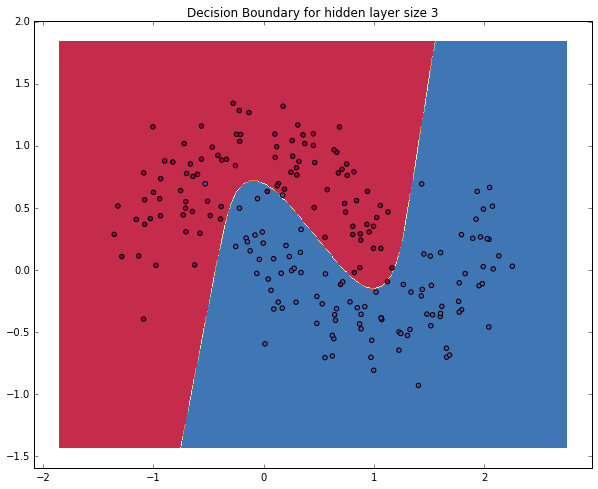
\includegraphics[width=0.5\textwidth]{result.png}
		\caption{预测结果}
		\label{fig:result}
	\end{figure}
\end{frame}

\section{图像分类}
\begin{frame}
	\begin{center}
		\vspace{0.1cm}
		\Huge{图像分类}
	\end{center}
\end{frame}

\subsection{AlexNet}
\begin{frame}
	\frametitle{ImageNet}
	\textbf{ImageNet数据集}: ImageNet 是一个按照 WordNet层次组织的图像数据库(目前只有名词).层次上的每个节点都有几百或几千个图像表示.目前,平均每个节点有超过5千张图像.\footnote{\label{ft:imagenet}http://www.image-net.org/}
\end{frame}
\begin{frame}
	\frametitle{ILSVRC2012}
	\textbf{ILSVRC2012}: 全称Large Scale Visual Recognition Challenge 2012.这个比赛的目的是利用人工标记的 ImageNet 的子集进行训练来判断照片中的内容,从而实现检索和自动标记.整体的目标是识别图像上出现的主要物体.\footnote{\label{ft:ilsvrc}http://image-net.org/challenges/LSVRC/2012/index}
\end{frame}
\begin{frame}
	\frametitle{AlexNet}
	ILSVRC2012图像分类冠军: ImageNet Classification with Deep Convolutional Neural Networks\autocite{krizhevsky2012imagenet}
\end{frame}
\begin{frame}
\begin{figure}
	\frametitle{AlexNet结构}
	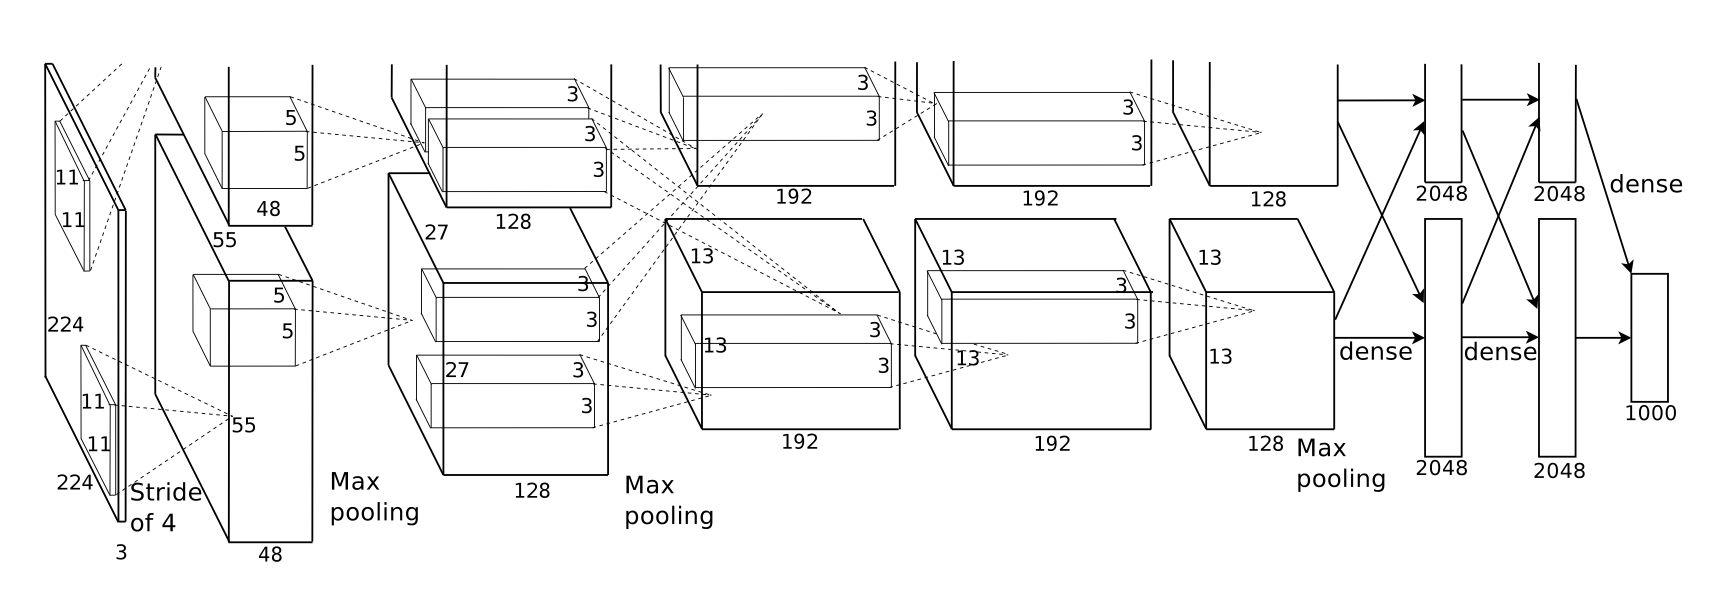
\includegraphics[width=0.8\textwidth]{AlexNet.png}
	\caption{AlexNet的CNN架构}
	\label{fig:alexnet}
\end{figure}
\end{frame}

\subsection{Demo}
\begin{frame}
	\frametitle{Demo}
	\begin{labeling}{alligator}
		\item [数据集] \textbf{Caltech256:} 包含从 Google 图像搜索和PicSearch.com上获得的 30, 607张物体的图像.这些图像通过人工判别被分配在257个类别中.
		\item [代码] 多伦多大学讲师 Michael Guerzhoy 在网站上提供了AlexNet 的 TensorFlow 实现及权重(weights). \footnote{\label{ft:alexnet}http://www.cs.toronto.edu/\textasciitilde{}guerzhoy/tf\_alexnet/}
	\end{labeling}
\end{frame}
\begin{frame}
	\frametitle{Caltech256图片示例-背包}
	\begin{figure}
		\centering
		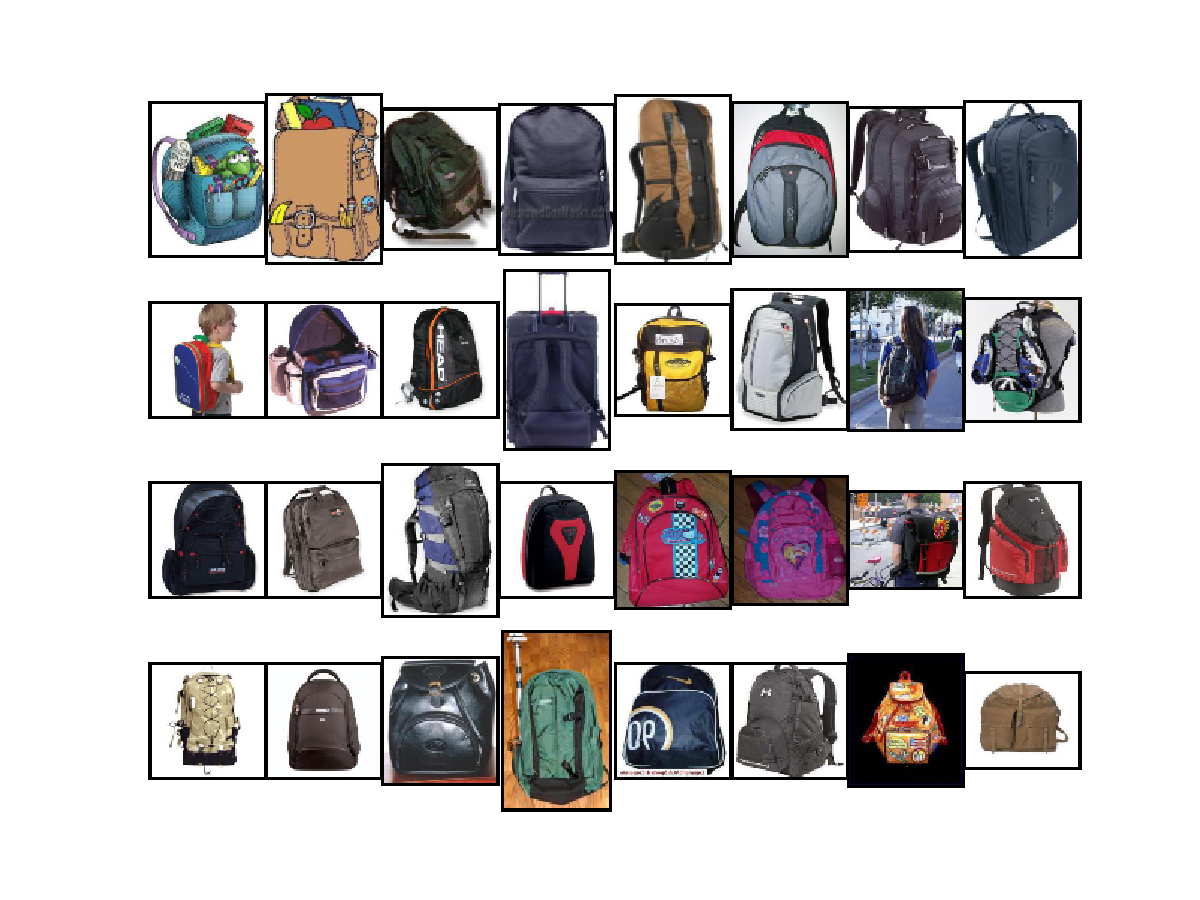
\includegraphics[width=0.7\linewidth]{backpack.pdf}
		\caption{背包}
	\end{figure}
\end{frame}
\begin{frame}
	\frametitle{Caltech256图片示例-咖啡杯}
	\begin{figure}
		\centering
		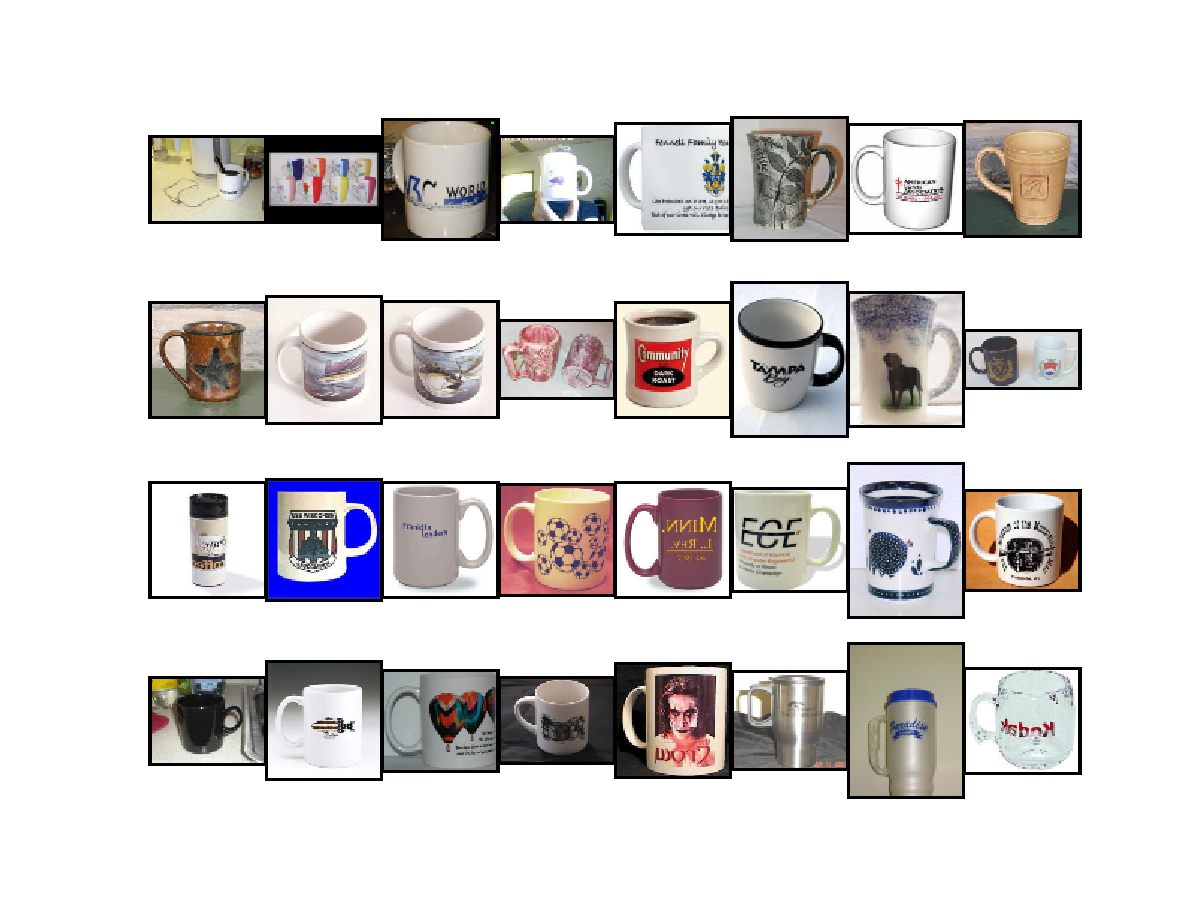
\includegraphics[width=0.7\linewidth]{coffee-mug.pdf}
		\caption{咖啡杯}
	\end{figure}
\end{frame}

\begin{frame}
	\begin{figure}
		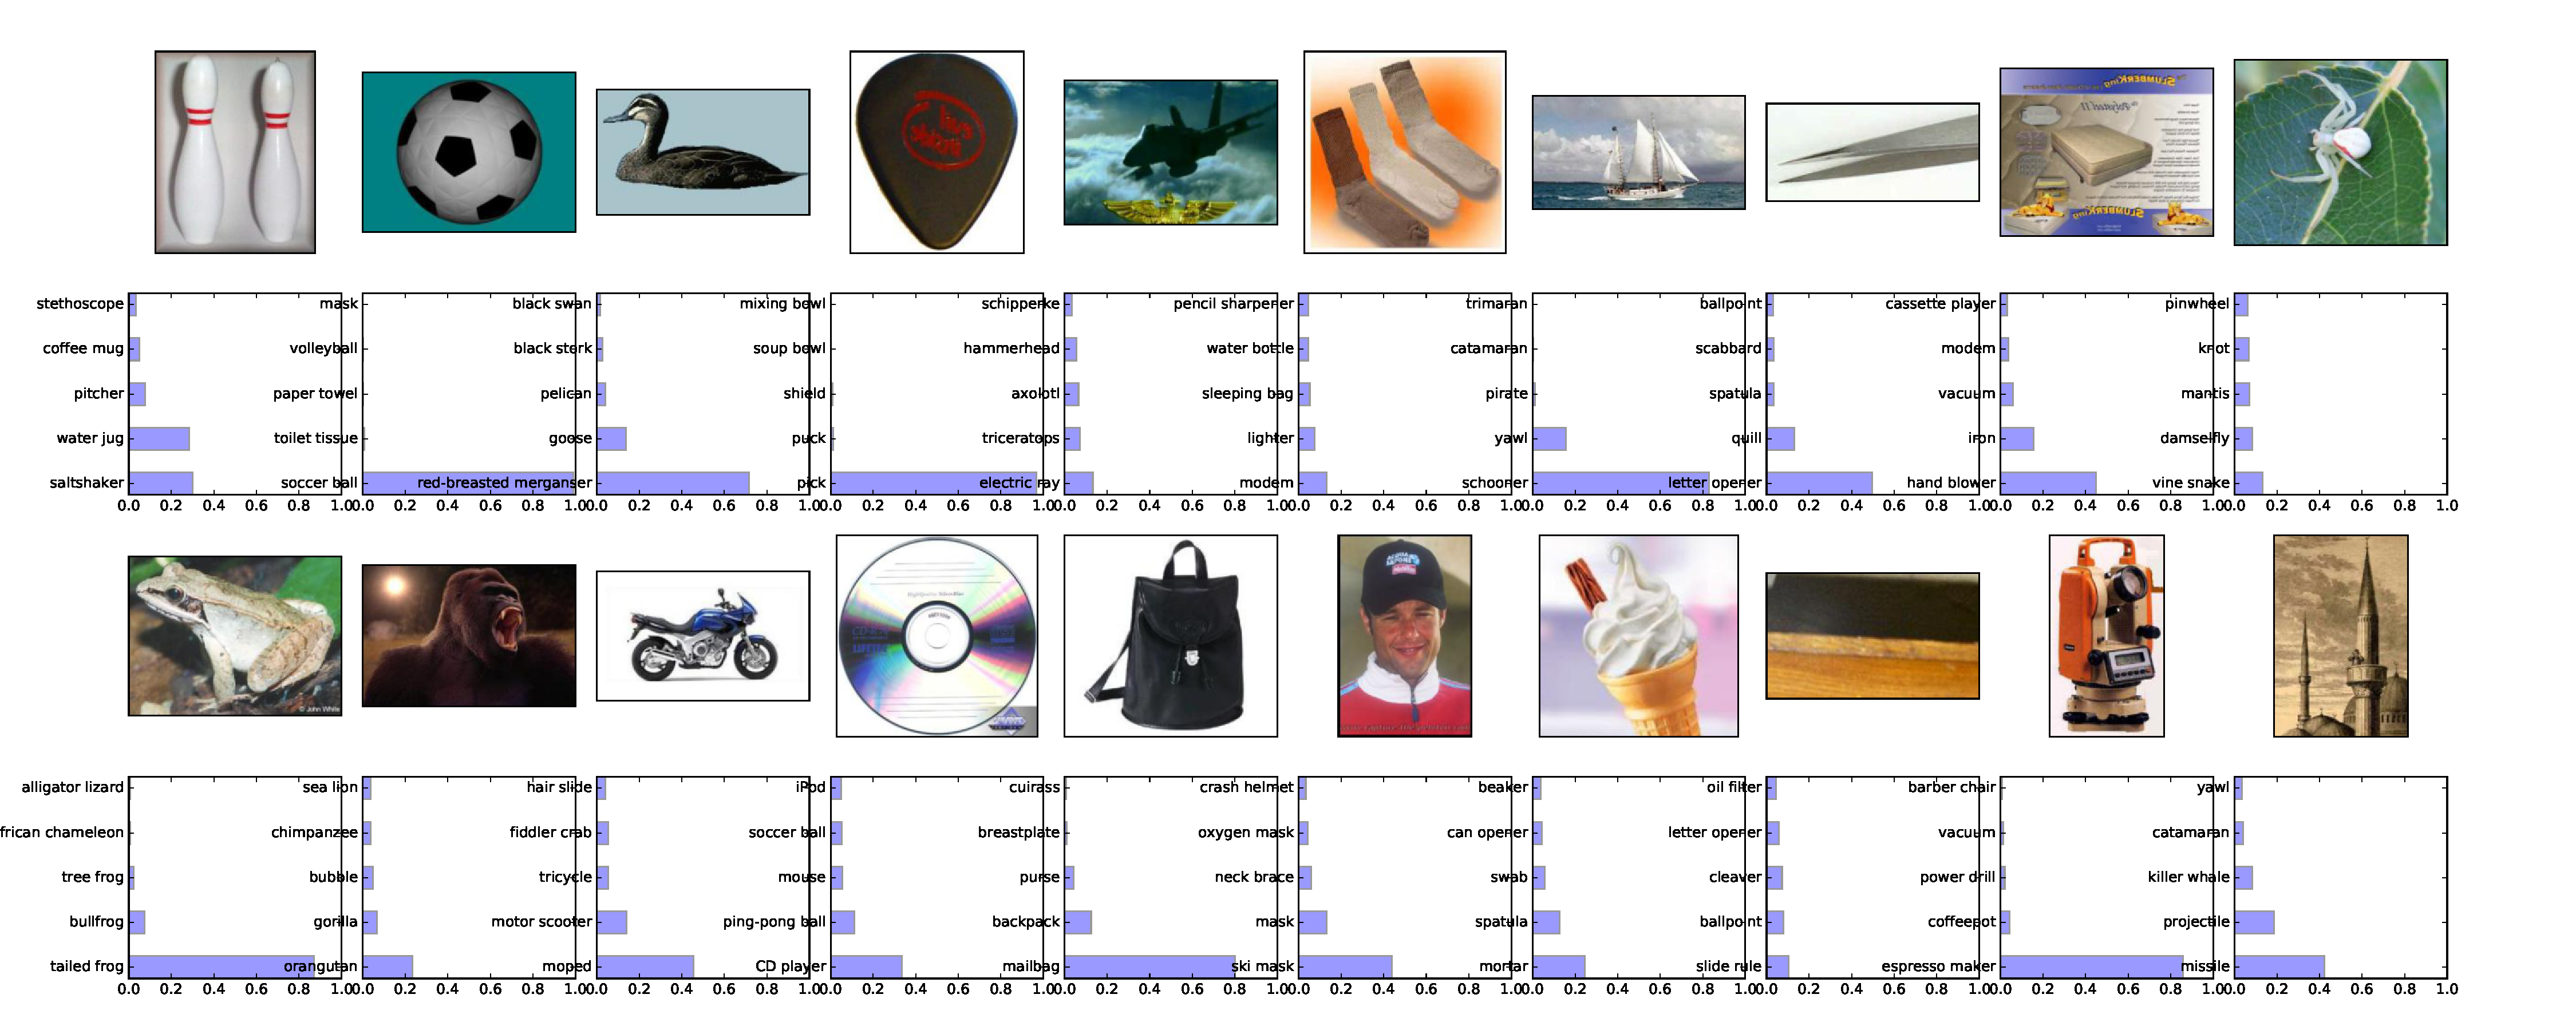
\includegraphics[width=\textwidth]{classification.pdf}
		\caption{分类结果}
		\label{fig:class}
	\end{figure}
	{\color{red}{现场演示(classification.py)......}}
\end{frame}

\begin{frame}
	\frametitle{技术前沿(State of the Art)}
	\begin{table}
		\begin{tabular}{|c|c|} \hline
			\rowcolor{gray!25} 模型 & Top 5 准确率 \\ \hline
			ResNet 152               & 92.92\%        \\ \hline
			ResNet 101               & 92.63\%        \\ \hline
			ResNet 50                & 92.02\%        \\ \hline
			VGG 16                   & 89.88\%        \\ \hline
			GoogLeNet                & 89.06\%        \\ \hline
			Network in Network       & 81.21\%        \\ \hline
			CaffeNet                 & 79.93\%        \\ \hline
			AlexNet                  & 79.84\%        \\ \hline
		\end{tabular}
		\caption{模型的准确率验证\footnote{https://github.com/ethereon/caffe-tensorflow}}
	\end{table}
\end{frame}

\section{图像检索}
\begin{frame}
	\begin{center}
		\vspace{0.1cm}
		\Huge{图像检索}
	\end{center}
\end{frame}
\subsection{企业应用实例}
\begin{frame}
	\frametitle{Pinterest}
	\tiny{Pinterest是一个网络与手机的应用程序,可以让用户利用其平台作为个人创意及项目工作所需的视觉探索工具,同时也有人把它视为一个图片分享类的社交网站,用户可以按主题分类添加和管理自己的图片收藏,并与好友分享.}\footnote{https://zh.wikipedia.org/wiki/Pinterest}
	\begin{figure}
		\includegraphics[width=0.9\textwidth]{pinterest.png}
		\caption{Pinterest网站}
		\label{fig:pinterest}
	\end{figure}
\end{frame}
\begin{frame}
	\frametitle{论文}
	\tiny{Pinterest在2014年收购了初创公司 VisualGraph,在它的平台上引入了视觉搜索. 在2015年,Pinterest发表了一篇论文Visual Search at Pinterest\autocite{jing2015visual},公开了它的系统架构:\footnote{https://en.wikipedia.org/wiki/Reverse\_image\_search}}
	\begin{itemize}
		\item Apache Hadoop
		\item Caffe卷积神经网络框架(AlexNet,VGG,Hamming Distance)
		\item Cascading(批量处理)
		\item PinLater(消息)
		\item Apache HBase(存储)
	\end{itemize}
	\begin{figure}
		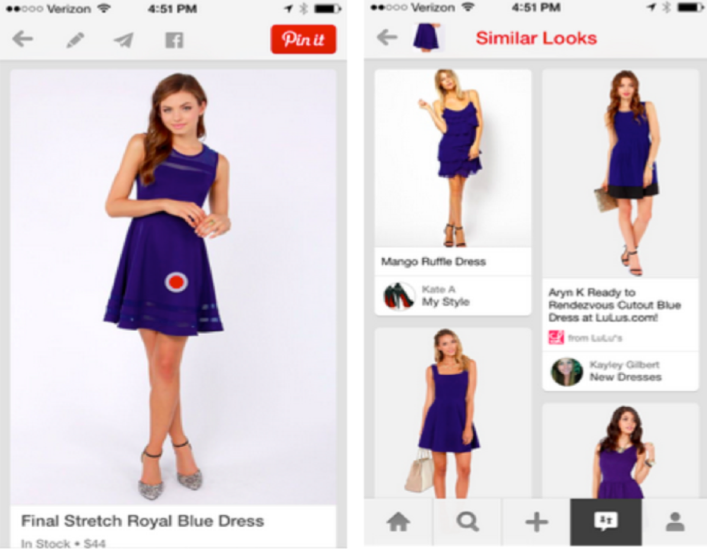
\includegraphics[width=0.4\textwidth]{Pinterest-Similar-Looks.png}
		\caption{用户一点击红点,系统会显示与检索物体相似的产品}
		\label{}
	\end{figure}
\end{frame}
\subsection{Demo}
\begin{frame}
	\frametitle{实验步骤}
	\begin{itemize}
		\item Caltech256数据集作为待检索的图片库
		\item 抽取AlexNet的fc6输出作为的图像的特征(4096维)
		\item 选择cosine作为图像特征之间距离(效果比欧式距离好)
		\item 检索时, 先抽取输入图像的特征, 计算与图片库中每个图像的距离, 然后排序
	\end{itemize}
	计算向量$u$与$v$之间的相关距离:
	\begin{equation}
		1 - \frac{u \cdot v}{||u||_2||v||_2}
	\end{equation}
\end{frame}
\begin{frame}
	\frametitle{实例}
	\begin{figure}
		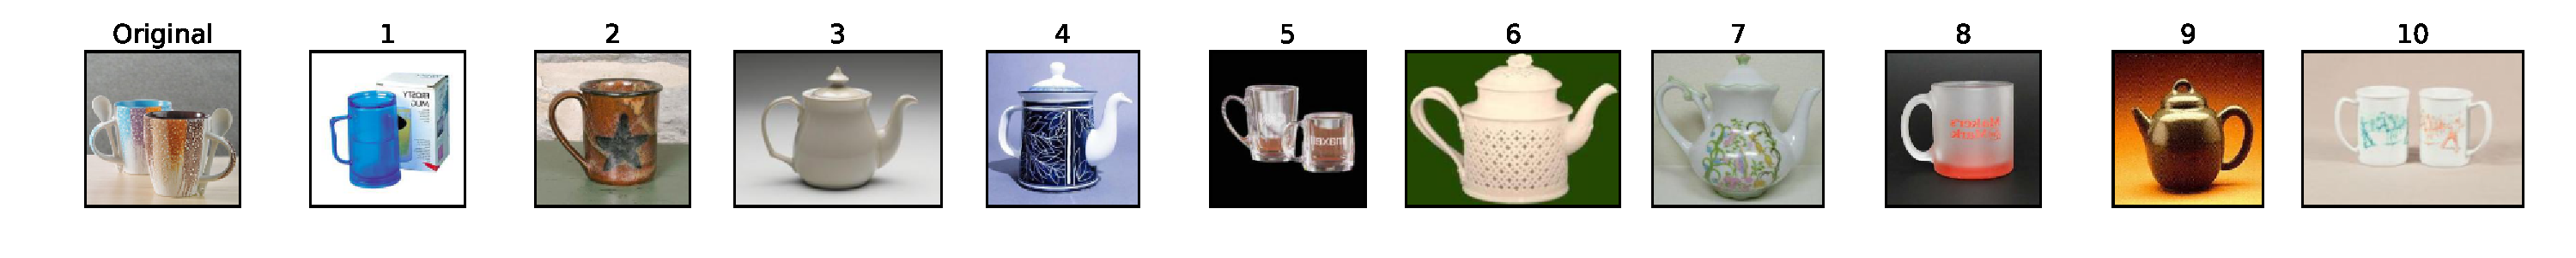
\includegraphics[width=\textwidth]{mug_search_result.pdf}
		\caption{图像检索实例}
		\label{}
	\end{figure}
\end{frame}
\begin{frame}
	\frametitle{图像变换检索实验}
	\begin{figure}
		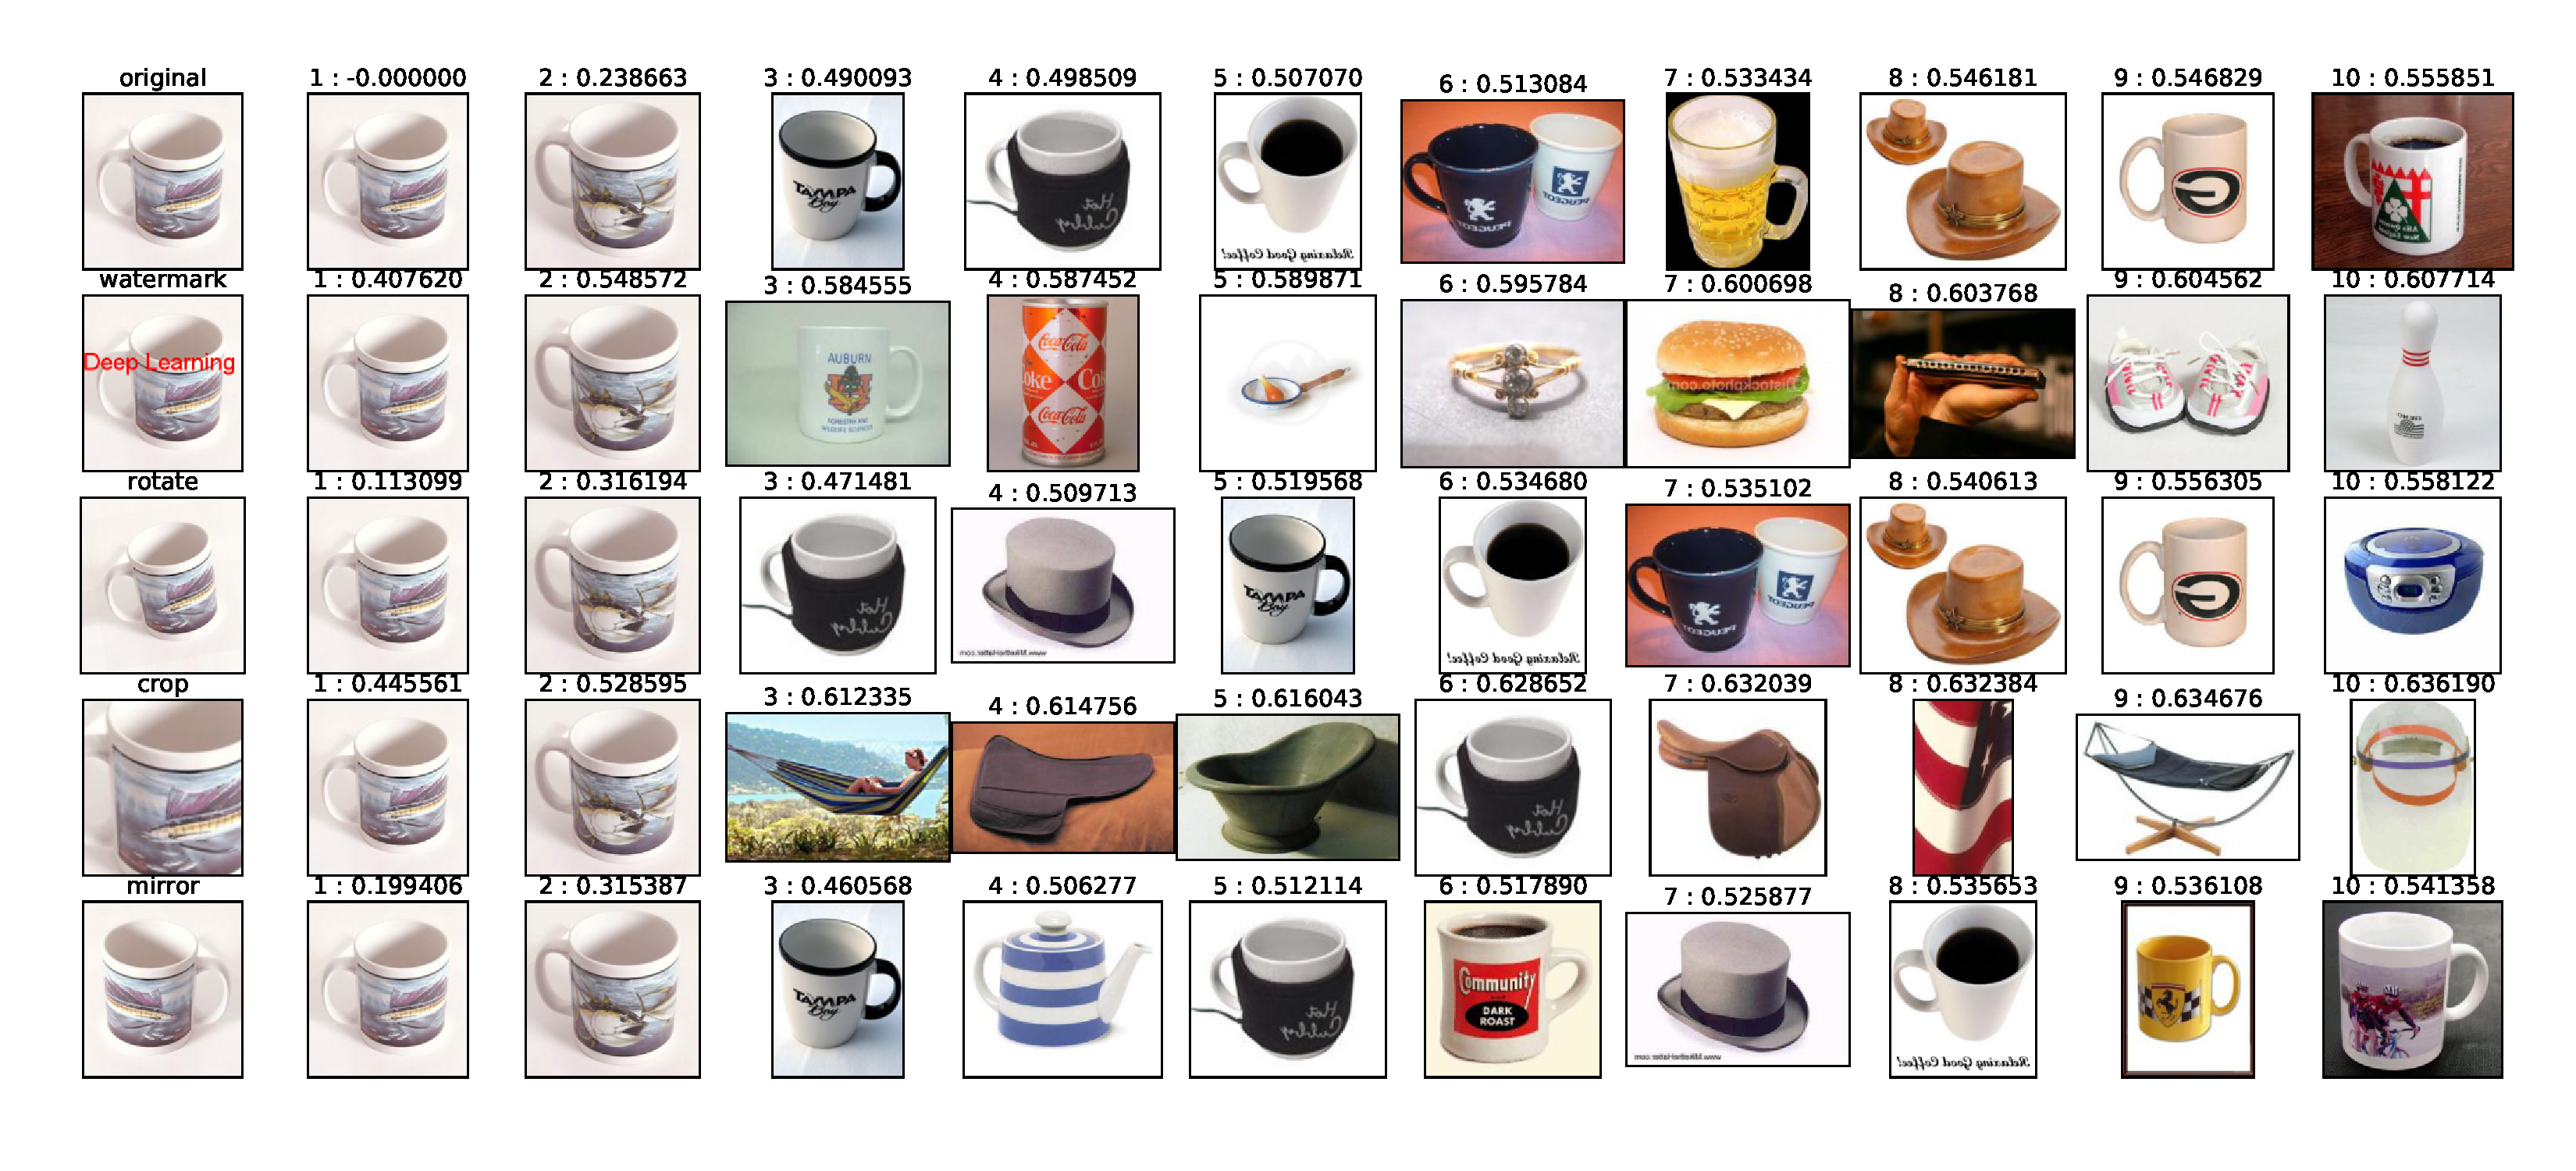
\includegraphics[width=\textwidth]{search_result.pdf}
		\caption{图像变换检索(文字水印,旋转(nearest),裁剪,镜像)}
		\label{}
	\end{figure}
	\tiny{速度(一次实验,非统计平均) query cost: 7.590151, dataset: 30185, query: 5}\\
	{\color{red}{现场演示(visual\_search.py)......}}
\end{frame}
\begin{frame}
	\frametitle{淘宝图片搜索}
	\begin{figure}
		\includegraphics[width=0.9\textwidth]{taobao_image_search.png}
		\caption{}
		\label{}
	\end{figure}
\end{frame}

\begin{frame}
	\frametitle{淘宝图像搜索存在的问题}
	搜索出来的商品类别与上传图片并不太一致, 比如上传一张马克杯图像, 返回结果排在前面的是保温杯, 茶具等.\\
	\textbf{可能的方案}: 先通过图像分类算法,识别物体类别,且在计算图片库特征时也按类别将图像分开, 在搜索时只搜索相关分类的图像,这样还能减少计算量,加快检索速度.
\end{frame}

\begin{frame}
	\frametitle{可以改进的地方}
	\begin{enumerate}
		\item 实验过程中对图像的预处理比较``粗暴''
		\item 特征相似度衡量方法的选择比较简单
		\item 检索时查询全库, 未做优化方面的探究
	\end{enumerate}
\end{frame}

\section*{}
\begin{frame}
	\begin{center}
		\vspace{0.1cm}
		\Huge{谢谢!}
	\end{center}
\end{frame}
%%-------------------------------------------------
\begin{frame}
	\frametitle{参考文献}
	\printbibliography[title={参考文献}]
\end{frame}
%%-------------------------------------------------


\end{document}
